% !TEX root =  ../thesis.tex

In this chapter we will talk about the overall design of the temporal profile analysis system. This system is based on the definition of user profiles for each time window, and then the analysis of how these profiles evolve in time.

\section{Overall system design}

The system, at a very high level, is composed of four main parts, as illustrated in figure~\ref{fig:system_design}.

First, transactions are grouped by time windows and user profiles are generated. One user profile is produced for each combination of user, time window and feature. For instance a profile could be associated with:\\ \texttt{user: 941825, time window: january 2015, feature: spent amount}.

Then, the distance from the past profiles is computed for each profile. The past is an average of the last few profiles for that user and feature, in the preceding time windows. This average is weighed on exponentially discounted weights the further in the past we go.

The third step is to analyze these distances and select anomalous ones, those that are greater than a dynamic threshold based on the standard deviation of past distances.

Lastly, after having identifies the profiles with anomalous distances, we select the transactions in these profiles that are the best candidates as to being responsible for the anomaly in the distances.

The final goal is to present these findings in a structured way to an expert analyst, detailing where each figure came from in the analysis, so that the analyst better know where to look and what to give more importance too also based on their experience.

\begin{figure}[h]
\centering
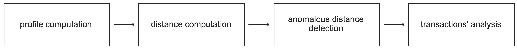
\includegraphics[width=450]{images/overall_system_design.pdf}
\caption{Overall system design of the temporal profile analysis system}
\label{fig:system_design}
\end{figure}

\section{Profiles and distances computation}

After a time window has passed (e.g.: the first of the month), the following procedure that creates the user profiles for the last time window and computes its distance is executed for each user. This process is illustrated in figure \ref{fig:distance_computation}.

\begin{enumerate}
  \item for each feature, a \textbf{profile} is built by creating the histogram representing the distribution of the values for that feature over all transactions in the last window. In figure \ref{fig:distance_computation} we build the profile for the amount feature. The amount is defined as a real number and divided into buckets based on its values and an interval defined for each bin.
  \item the exponentially discounted average of the past profiles is computed, defined as the average of the value of each bin in the last $N$ profiles, with weights exponentially discounted the more we go further in to the past. All histograms have the same number of bins, and so does the average histogram.
  \item the distance between the current profile and the \textbf{average} profile is computed, following the distance rules associated with this feature. In the example of the amount, we have an ordinal histogram, therefore we use our definition of distance that applies a smoothing filter and an euclidean distance. If we were analyzing the feature \texttt{hour of the day}, which generates a modulo histogram, we would have used the modulo distance (where the smoothing filter is circular). Lastly, for nominal features such as \texttt{type} we would have used directly the euclidean distance.
\end{enumerate}

\begin{figure}[h]
\centering
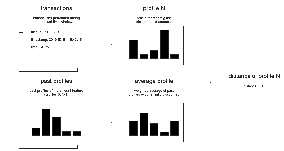
\includegraphics[width=450]{images/distance_computation.pdf}
\caption{Overall system design of the temporal profile analysis system}
\label{fig:distance_computation}
\end{figure}

\section{Anomalous distance detection}

At this stage we have, for a combination of user and feature, a chronological series of profiles (one for each time window). For each profile, we know its distance from the past, how much that profile changed compared to the past ones. This represents a shift in spending habits of the user, who maybe began working at night or spending larger sums, or whose transactions might in fact be frauds.

The current step identifies the profiles whose distance is greater than normal. How do we define the threshold for normality? The standard deviation of the $M$ previous distances, where $M$ is a tunable parameter, is computed. The threshold is dynamically defined for each profile as this standard deviation times a sensitivity parameter $\alpha$. In this way, we can mark as anomalous only those profile that move apart from the current mean by more than $\alpha$ times the typical standard deviation.

The following procedure summarizes what we have just explained, and is illustrated in figure \ref{fig:distance_analysis}:

\begin{enumerate}
  \item the \textbf{standard deviation} of the $M$ previous distances is computed, where $M$ is a parameter to be chosen
  \item the \textbf{anomaly} of the current profile is computed as:
    \begin{displaymath}
      \frac{\text{distance}-\text{average distance}}{\text{std dev of previous distances}}
    \end{displaymath}
  \item profiles with an anomaly level greater than a \textbf{threshold} $\alpha$ to be chosen are notified to the analyst
\end{enumerate}

\begin{figure}[h]
\centering
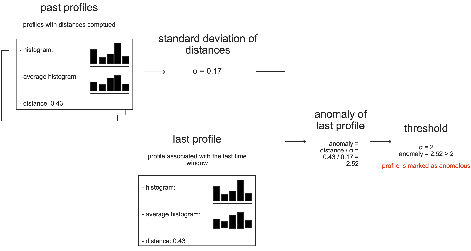
\includegraphics[width=450]{images/distance_analysis.pdf}
\caption{Analysis of the distances between profiles to determine anomalous profiles}
\label{fig:distance_analysis}
\end{figure}

\section{Transactions' analysis}
\label{sec:transactions_analysis}

The last step of our system is to try to identifies those transactions part of the anomalous profiles that could be responsible for such anomaly. For example, if we have an anomalous profiles for the feature amount, we select those features that were the most atypical in terms of amount, in a similar way to what is done in the local profile in BankSealer \cite{banksealer}.

While this might seem redundant with respect to the local profile at first, what it does is very different. Transactions are not marked as anomalous because individually they differed from the typical user behaviors, but because they contribute to an overall behavioral shift. This is to be combined with the information we get form the local profile, so that fraudulent transactions that ordinarily would have passed by the local profile can be brought up by our temporal analysis.

To select the interesting transactions we have adopted a simple approach: search for bins which diverge the most from the average, and take those transactions as interesting. We stop when the distance, recomputed without considering these bins, falls under the anomaly threshold.

We will explain this in more detail in the next paragraphs, but first an important element to be considered is anomaly caused by absence rather than presence. Distance is symmetric, and the same anomaly level can be caused by an increment in transactions (for instance, with amount around 500 euros) and by a decrement of such transactions. It is however impossible to collect transactions that contributed to the anomaly if a decrement happened, and also less likely that the problem is associated with an attempted fraud.

The procedure (illustrated in figure \ref{fig:transactions_analysis}) is as follows:

\begin{enumerate}
  \item we sort the bins of the last histogram in decrescent order by the absolute difference of their values compared to the average histogram.
  \item we take the first bin. If its value is greater than the one in the average histogram, we select as interesting all the transactions in the bin. If it's lower, we mark the bin as anomalous because of absence.
  \item we recompute the distance without considering the previous bin (practically, we do this setting it to the same value as the corresponding bin in the average histogram). If the distance is still above the threshold of anomaly, we start over at step 1, otherwise we have finished collecting interesting transactions.
\end{enumerate}

\begin{figure}[h]
\centering
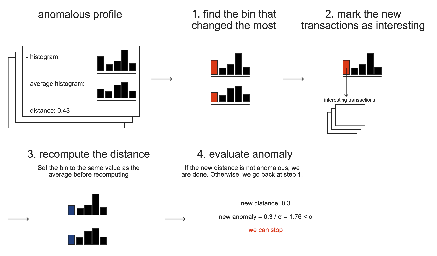
\includegraphics[width=450]{images/transactions_analysis.pdf}
\caption{Algorithm to find the most interesting transactions in an anomalous profile}
\label{fig:transactions_analysis}
\end{figure}
